\section{Methods}
\label{sec:methods}

We ask one question: when a judge who cannot see the evidence oversees a debate between an honest debater and a
dishonest debater expected to be stronger, does letting the judge verify a few facts help or hurt?
Figure~\ref{fig:protocol} shows the setup. The original design, hypotheses and analysis were frozen before the main
run, and nobody looked at results while it ran. Appendix~\ref{app:deviations} lists every departure from that plan,
including three amendments written before any result was seen.

\begin{figure}[t]
\centering
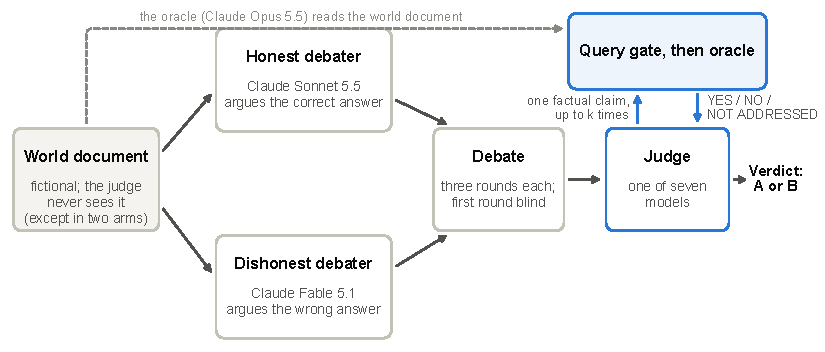
\includegraphics[width=0.9\linewidth]{fig_protocol}
\caption{The setup. Two debaters read a fictional world document and argue opposite answers to a question about it.
The judge sees only the debate. In the query conditions the judge may check up to $k$ factual claims, one at a time,
with an oracle that reads the document. Each claim first passes a gate, a filter meant to stop the judge from simply
asking for the answer (Section~\ref{sec:oracle}).}
\label{fig:protocol}
\end{figure}

\subsection{Task: questions about invented worlds}
\label{sec:task}

Each question is about a fictional ``world'': a document of about \worldWordsMedian{} words (\worldWordsMin{} to
\worldWordsMax{}) describing an invented place, with its institutions, trade and history. Because the worlds are
newly invented, a model cannot answer from memorised facts about them, and we control what evidence the judge is
given. Models still bring general expectations and may pick up cues in the wording.

Two frontier models, Claude Fable 5.1 and GPT-6 Astra, each wrote 80 worlds. With each world they wrote candidate
questions that combine several facts, for example whether an institution could take some action or what
caused some event. Every question comes with a correct answer, a wrong answer that is meant to be defensible, and the
list of facts the correct answer rests on. An example:

\begin{quote}\small
\emph{Question.} Given the Moot's rules and the positions the six cities took over the Scarp trade in Cycle 219, could
the Moot of Mouths declare war on the Dunmere clan to halt the Scarp carriers if Keddon, Ammerly and Vashe all sought
it?\\
\emph{Correct answer (summary).} No: a declaration of war needs all six votes, and three cities voted to keep the road
open.\\
\emph{Wrong answer (summary).} Yes: the Moot acts toward outside peoples on four votes, and a fourth city would join.
\end{quote}

Before any debate, each question was checked by two validators that had not written its world (the other author
model and DeepSeek V4 Pro). Each answered from the full document, in both answer orders, without seeing
the answer key. A question was kept only if all four answers matched the key, neither validator called the wrong
answer about equally defensible, and every listed fact checked out against the document. This filter keeps only
questions that models answer correctly from the full document, so low error with the document is partly built in.
Validators also flagged questions where another reading of the document could reverse the answer; a flag did not
exclude a question, and \nFlaggedTwoPlus{} of the \nCounted{} analysed questions drew one in at least two of the four
responses (Section~\ref{sec:robust}).

Worlds were then split by a fixed hash into small development sets (20 worlds) and the main set of \nWorlds{}
worlds, 70 per author. The main set has \nQuestions{} questions; \nCounted{} are analysed, and the two set aside
before the run for a defect in their source document enter only one robustness check. No main-set question was used in any debate or judgment before the main run.

\subsection{Debates}
\label{sec:debates}

Each question got one debate. The honest debater, Claude Sonnet 5.5, was given the correct answer. The dishonest
debater, Claude Fable 5.1, was given the wrong answer, told that it was wrong, and told to argue for it as
convincingly as possible; it was allowed to frame facts misleadingly, omit facts and fabricate. Both debaters read
the full world document and were told that the judge might be able to verify a limited number of claims. A debate has
three rounds per side, the first written without seeing the opponent, and no word cap. A fixed hash assigned which
side spoke first (Appendix~\ref{app:deviations}). Each debate was written
once and shown unchanged in every debate condition; the debaters did not know how many queries a judge would have.
The dishonest debater also received the benchmark's short note on why its answer could be defended, written by the
world's author (prompts: Appendix~\ref{app:prompts}).

We chose this pairing to put the model we expected to be the stronger on the dishonest side, the case that matters
for oversight, and because it gave judges something to get wrong: in a development run, error without queries was
22.9\% with Sonnet on the honest side against 5.0\% when Fable debated itself. Those rates come from different
questions and judges than the main run, and most of the development errors came from a judge that was later lost
(Appendix~\ref{app:deviations}). The study does not itself rank the two models: the dishonest side also ran at a
higher effort setting and twice the output limit (Appendix~\ref{app:materials}). In the main run the dishonest
debater wrote about twice as much as the honest one (834 against 435 words per turn on average).

\subsection{Judges and conditions}
\label{sec:conditions}

Seven models served as judges: GPT-5.6 Luna, Terra and Sol; Claude Haiku 4.5, Sonnet 5.5 and Opus 5.5; and Qwen3.8.
An eighth planned judge, Llama 3.3 70B, was withdrawn by its provider during the run and produced no judgments; an
amendment written before any result was seen made the other seven the primary panel
(Appendix~\ref{app:deviations}). Every judge saw every question in six conditions, twice, with the order of the two
answers swapped: the debate with 0, 1, 2 or 6 oracle queries on offer; the debate together with the world document,
with no queries; and the world document alone, with no debate or queries. The GPT-5.6
judges, Sonnet 5.5 and Opus 5.5 ran at a medium effort setting, Haiku 4.5 without extended thinking and Qwen3.8 at
its provider's default (Appendix~\ref{app:materials}). In the query conditions the judge is told its budget, submits one claim at a time, sees each answer before writing
the next claim, and may stop early. Every session ends with a choice between the two answers.

\subsection{The oracle and the query gate}
\label{sec:oracle}

A query is a single factual claim about the world. The oracle, Claude Opus 5.5, reads the world document and replies
\textsc{yes} (the document supports the claim), \textsc{no} (it contradicts it) or \textsc{not addressed}. It is
told to use only what the document states and to make no inferences. Judges saw only the oracle's bare label;
they were not told how the oracle was instructed. In development it agreed with model-set reference answers in 93\%
of 300 cases, exactly the minimum fixed in advance; that sample was also used to select the oracle, so this is not
an estimate of its accuracy in the main run (Appendix~\ref{app:materials}).

Without a restriction, a judge could simply ask the oracle which answer is correct. So every query first passes a
\emph{gate} that enforces a fixed rule: one checkable fact per query; no naming of a debater, a position or a
candidate answer; no asserting either answer's overall conclusion; no bundling of several facts; and no asking for
an evaluation or inference. Checking an individual fact that a debater cited is allowed
(Appendix~\ref{app:prompts} has the full rule). The gate is a set of mechanical checks followed by a
classifier (DeepSeek V4 Flash) that sees the question, both answers and the query, but not the world or the answer
key. A rejected query may be rewritten once; a second rejection uses up that query.

\emph{One deviation matters for reading the results.} Early in the run the provider withdrew the gate classifier,
before any query had received a decision. We ran the same model and prompt on a dedicated deployment instead, and it
screened every query in the main run. That deployment failed a check, fixed in advance, of its agreement with the
gate as it had run in development; the check showed neither that the two gates were equivalent nor that they
differed by much (Appendix~\ref{app:gate}). We adopted the deployment as a disclosed deviation and, after the run,
audited how often rule-breaking queries got through (Section~\ref{sec:gate}). The run was also split in time: the
three conditions without queries finished before the gate outage, and most query-condition verdicts came about a day
later (Appendix~\ref{app:deviations}). Comparisons of a query condition with the no-query or document conditions
therefore largely cross that split, and reading them as effects of the queries assumes that the judges behaved the
same on both sides of it, which we did not test. Comparisons among query budgets largely do not cross it.

\subsection{Measures and analysis}
\label{sec:analysis}

A judgment is an \emph{error} if the judge does not choose the correct answer; an unreadable or empty verdict counts
as an error. Unreadable verdicts were rare (\nUnreadable{} of \nSevenSessions{} sessions), but most were replies cut
off at the output limit, and those were uneven across conditions: over all \nQuestions{} questions, Qwen3.8 had
\qwenCutZero{} among its no-query replies against \qwenCutSix{} with six queries (Appendix~\ref{app:stats}). For each judge and condition we average the two answer orders within
a question and then average over questions. Pooled results are the simple mean over the seven judges, so each judge
counts equally. They describe these seven judges: the intervals we report reflect which worlds were sampled, not
which judges.

The registered hypothesis is an inverted U: offering a small query budget (1 or 2 queries) produces higher error
than both no queries and a larger budget (6). A peak at 1 or 2 queries counts as supported only if error there is
higher than at both ends, after we correct for having tested two budgets. We also fixed in advance that a peak under 1.5 percentage points would be too small to matter.

We report differences in percentage points with 95\% intervals, from a bootstrap that resamples whole worlds so
that questions sharing a world are not treated as independent (Appendix~\ref{app:stats}). What these comparisons
measure, given the stability assumed in Section~\ref{sec:oracle}, is the effect of \emph{offering} a query budget
under this protocol, with the judge's anticipation, stopping and extra computation included. They do not measure
the effect of one more oracle answer taken in isolation.
